% =============================================================================
% RELATÓRIO TÉCNICO-ACADÊMICO — ETAPA 1 (DISCIPLINA DE BANCO DE DADOS)
% Padrão ABNT (abntex2 + abntex2cite [alf]) — Compatível com TeX Live e Overleaf
% =============================================================================
\documentclass[
    12pt,
    openany,
    oneside,
    a4paper,
    english,
    brazil
]{abntex2}

% --- Pacotes de codificação, fontes e tipografia ---
\usepackage{cmap}
\usepackage[T1]{fontenc}
\usepackage[utf8]{inputenc}
\usepackage{lmodern}
\usepackage{indentfirst}
\usepackage{microtype}

% --- Pacotes gráficos, tabelas e citações ---
\usepackage{graphicx}
\usepackage{booktabs}
\usepackage{array}
\usepackage{xcolor}
\usepackage{csquotes}
\usepackage{hyperref}
\usepackage[alf,abnt-emphasize=bf]{abntex2cite}

% --- Tipos de coluna alinhados à esquerda/direita sem hifenização forçada ---
\newcolumntype{L}[1]{>{\raggedright\arraybackslash}p{#1}}
\newcolumntype{R}[1]{>{\raggedleft\arraybackslash}p{#1}}

% --- Configuração de margens ABNT (NBR 14724): sup/esq 3 cm; inf/dir 2 cm ---
\setlrmarginsandblock{3cm}{2cm}{*}
\setulmarginsandblock{3cm}{2cm}{*}
\checkandfixthelayout

% --- Espaçamento de parágrafos, seções e indentação ABNT ---
\setlength{\parindent}{1.25cm}
\setlength{\parskip}{0pt}
\setlength{\afterchapskip}{18pt}
\setlength{\beforesecskip}{14pt}
\setlength{\aftersecskip}{8pt}
\setlength{\beforesubsecskip}{10pt}
\setlength{\aftersubsecskip}{6pt}

% --- Dados do grupo, disciplina e instituição ---
% =============================================================================
% DADOS DO GRUPO E DA DISCIPLINA (PLACEHOLDERS SIMBÓLICOS PARA EDIÇÃO MANUAL)
% Edite apenas este arquivo para atualizar a capa e a folha de rosto.
% =============================================================================
\newcommand{\instituicaoNome}{{[NOME DA INSTITUIÇÃO]}}
\newcommand{\cursoNome}{{[CURSO]}}
\newcommand{\disciplinaNome}{Banco de Dados}
\newcommand{\professorNome}{{[PROFESSOR(A)]}}
\newcommand{\cidadeLocal}{{[CIDADE]}}
\newcommand{\anoTrabalho}{2026}
\newcommand{\tituloTrabalho}{Monitoramento e Manutenção Colaborativa de Infraestrutura Urbana: Descrição do Problema, Enquadramento nos ODS e Escopo do Sistema de Banco de Dados}
% Integrantes: formato "Nome Completo --- RA 000000"
\newcommand{\integrantes}{%
  {[NOME 1]} --- RA {[RA 1]}\\
  {[NOME 2]} --- RA {[RA 2]}\\
  {[NOME 3]} --- RA {[RA 3]}%
}


\titulo{\tituloTrabalho}
\autor{\integrantes}
\local{\cidadeLocal}
\data{\anoTrabalho}
\instituicao{%
  \instituicaoNome
  \par
  \cursoNome
  \par
  Disciplina: \disciplinaNome
}
\orientador[Professor(a):]{\professorNome}
\preambulo{Trabalho acadêmico apresentado à disciplina de \disciplinaNome{} do curso de \cursoNome{} da \instituicaoNome{}, como requisito parcial de avaliação da Etapa 1 (Descrição do Problema e Enquadramento nos Objetivos de Desenvolvimento Sustentável).}

% --- Customização da Capa ABNT (NBR 14724) para incluir Instituição no topo ---
\renewcommand{\imprimircapa}{%
  \begin{capa}%
    \center
    {\ABNTEXchapterfont\large\imprimirinstituicao}
    \vspace*{1.5cm}

    {\ABNTEXchapterfont\large\imprimirautor}

    \vfill
    \begin{center}
    \ABNTEXchapterfont\bfseries\LARGE\imprimirtitulo
    \end{center}
    \vfill

    \large\imprimirlocal

    \large\imprimirdata

    \vspace*{1cm}
  \end{capa}
}

% --- Configurações do pacote hyperref (PDF/Metadados) ---
\definecolor{blueLink}{RGB}{0,51,102}
\makeatletter
\hypersetup{
    pdftitle={\tituloTrabalho},
    pdfauthor={Grupo - Disciplina de Banco de Dados},
    pdfsubject={Monitoramento e Manutenção Colaborativa de Infraestrutura Urbana (ODS 11)},
    pdfkeywords={Infraestrutura urbana, Zeladoria municipal, Banco de dados relacional, ODS 11, Agenda 2030},
    colorlinks=true,
    linkcolor=black,
    citecolor=black,
    filecolor=black,
    urlcolor=blueLink,
    bookmarksdepth=4
}
\makeatother

% =============================================================================
% INÍCIO DO DOCUMENTO
% =============================================================================
\begin{document}

\selectlanguage{brazil}
\frenchspacing

% -----------------------------------------------------------------------------
% ELEMENTOS PRÉ-TEXTUAIS
% -----------------------------------------------------------------------------
\pretextual

% Capa (sem conflito de âncora hyperref page.1 com a folha de rosto)
\hypersetup{pageanchor=false}
\imprimircapa
\hypersetup{pageanchor=true}

% Folha de rosto (início da contagem de páginas ABNT NBR 14724)
\imprimirfolhaderosto*

% Resumo em língua vernácula (Português) e língua estrangeira (Inglês)
\begin{resumo}
\begin{SingleSpacing}
A conservação contínua da infraestrutura urbana constitui um desafio estrutural para a administração pública de municípios brasileiros de médio e grande porte, nos quais falhas cotidianas --- como buracos na pavimentação asfáltica, lâmpadas de iluminação pública inoperantes, obstruções ou vazamentos em redes de drenagem pluvial, semáforos defeituosos e pontos de descarte irregular de resíduos sólidos --- comprometem a segurança viária, a salubridade ambiental e o bem-estar coletivo. Na maioria das prefeituras, o fluxo informacional entre o cidadão que vivencia o problema no território e as equipes operacionais encarregadas do reparo caracteriza-se pela fragmentação, gerando chamados duplicados, imprecisão na localização geográfica das ocorrências, ausência de evidências visuais padronizadas e falta de controle sobre o despacho de frota, a alocação de mão de obra e o consumo de insumos de almoxarifado. Diante desse cenário, este relatório técnico-acadêmico, referente à Etapa 1 do projeto da disciplina de Banco de Dados, tem como objetivo descrever detalhadamente o problema da gestão colaborativa de zeladoria e manutenção de infraestrutura urbana, fundamentar seu enquadramento nos Objetivos de Desenvolvimento Sustentável (ODS) da Agenda 2030 da Organização das Nações Unidas (ONU) e delimitar o escopo funcional de um sistema de banco de dados relacional voltado à sua resolução. A análise apoia-se em dados oficiais do Instituto Brasileiro de Geografia e Estatística (IBGE), do Instituto de Pesquisa Econômica Aplicada (IPEA), do Sistema Nacional de Informações sobre Saneamento (SNIS) e da legislação nacional de gestão urbana e defesa do usuário do serviço público. Demonstra-se que a proposta se alinha diretamente ao ODS 11 (Cidades e Comunidades Sustentáveis), com ênfase nas Metas 11.3, 11.6 e 11.7, e de modo complementar ao ODS 9 (Indústria, Inovação e Infraestrutura, Meta 9.1) e ao ODS 16 (Paz, Justiça e Instituições Eficazes, Metas 16.6 e 16.7). Por fim, estabelece-se o escopo de alto nível do banco de dados composto por doze entidades de negócio organizadas em três subdomínios integrados --- demandas cidadãs geolocalizadas por CEP, estrutura operacional das secretarias municipais e execução de ordens de serviço articulada à cadeia de suprimentos ---, preparando a base conceitual para a modelagem entidade-relacionamento e relacional desenvolvida na Etapa 2.

\vspace{\onelineskip}
\noindent
\textbf{Palavras-chave}: Infraestrutura urbana. Zeladoria municipal. Banco de dados relacional. Objetivos de Desenvolvimento Sustentável. ODS 11.
\end{SingleSpacing}
\end{resumo}

\begin{resumo}[Abstract]
\begin{otherlanguage*}{english}
\begin{SingleSpacing}
Continuous maintenance of urban infrastructure represents a structural challenge for public administration in medium- and large-sized Brazilian municipalities, where everyday failures --- such as potholes in asphalt paving, non-functional public lighting poles, blockages or leaks in stormwater drainage networks, malfunctioning traffic lights, and irregular solid waste disposal sites --- compromise road safety, environmental health, and collective well-being. In most municipal governments, the information flow between citizens who identify problems in the territory and operational field teams responsible for repairs is fragmented, resulting in duplicate service requests, imprecise geographic location data, lack of standardized visual evidence, and insufficient control over fleet dispatch, workforce allocation, and warehouse material consumption. Given this context, this technical and academic report, corresponding to Stage 1 of the Database course project, aims to describe in detail the problem of collaborative urban infrastructure monitoring and maintenance, substantiate its alignment with the United Nations (UN) 2030 Agenda Sustainable Development Goals (SDGs), and define the functional scope of a relational database system designed to address it. The analysis is grounded in official data from the Brazilian Institute of Geography and Statistics (IBGE), the Institute for Applied Economic Research (IPEA), the National Sanitation Information System (SNIS), and Brazilian federal legislation on urban management and public service user rights. The study demonstrates that the proposed solution aligns directly with SDG 11 (Sustainable Cities and Communities), specifically Targets 11.3, 11.6, and 11.7, and complementarily with SDG 9 (Industry, Innovation and Infrastructure, Target 9.1) and SDG 16 (Peace, Justice and Strong Institutions, Targets 16.6 and 16.7). Finally, the high-level scope of the database is established across twelve business entities organized into three integrated subdomains --- citizen demands geolocated by postal code (CEP), municipal secretariat operational structure, and work order execution linked to the supply chain --- providing the conceptual foundation for the entity-relationship and relational modeling developed in Stage 2.

\vspace{\onelineskip}
\noindent
\textbf{Keywords}: Urban infrastructure. Municipal maintenance. Relational database. Sustainable Development Goals. SDG 11.
\end{SingleSpacing}
\end{otherlanguage*}
\end{resumo}


% Lista de ilustrações (figuras)
\pdfbookmark[0]{\listfigurename}{lof}
\listoffigures*
\newpage

% Lista de tabelas
\pdfbookmark[0]{\listtablename}{lot}
\listoftables*
\newpage

% Sumário
\pdfbookmark[0]{\contentsname}{toc}
\tableofcontents*
\newpage

% -----------------------------------------------------------------------------
% ELEMENTOS TEXTUAIS
% -----------------------------------------------------------------------------
\textual

\chapter{Introdução}
\label{cap:introducao}

O processo de urbanização brasileiro consolidou, ao longo das últimas décadas, uma expressiva concentração demográfica nos centros urbanos. De acordo com os resultados do Censo Demográfico 2022, apurados pelo \citeonline{ibge2024censo2022malha}, cerca de 177,5 milhões de habitantes residem em áreas urbanas no Brasil, o que corresponde a 87,4\% da população total do país, estimada em 203,1 milhões de pessoas. Esse adensamento populacional exerce pressão contínua sobre os equipamentos e as redes físicas que sustentam a vida cotidiana nos municípios de médio e grande porte, exigindo da administração pública local ações permanentes de conservação, reparo e monitoramento do espaço urbano.

No exercício diário da gestão municipal, o conjunto de atividades voltadas à conservação das vias e dos equipamentos coletivos --- comumente denominado zeladoria urbana --- abrange serviços essenciais como a manutenção da pavimentação asfáltica, a operação da rede de iluminação pública, a desobstrução e o reparo de galerias de drenagem pluvial, o funcionamento da sinalização semafórica e a remoção de pontos de descarte irregular de resíduos sólidos. Quando essas infraestruturas sofrem degradação e não recebem intervenção tempestiva, instalam-se externalidades negativas imediatas que afetam a mobilidade, a segurança viária, a saúde pública e a valorização do patrimônio coletivo \cite{ibge2025entorno, snis2023drenagem}.

Apesar da relevância crítica desses serviços, o fluxo de comunicação e de gestão operacional predominante na maioria das prefeituras brasileiras ainda opera de maneira fragmentada e reativa. De um lado, o cidadão que identifica uma falha de infraestrutura em seu bairro encontra canais de atendimento dispersos, frequentemente desprovidos de padronização geográfica por Código de Endereçamento Postal (CEP) e incapazes de receber registros fotográficos ou audiovisuais que comprovem a gravidade da situação. De outro lado, os órgãos e secretarias municipais enfrentam dificuldades para consolidar demandas repetidas sobre um mesmo logradouro, planejar o deslocamento de suas equipes de manutenção e veículos de frota, controlar o consumo de materiais de almoxarifado adquiridos junto a fornecedores externos e aferir a efetiva resolução do problema junto ao solicitante.

A superação dessas lacunas informacionais relaciona-se diretamente aos compromissos globais pactuados na Agenda 2030 para o Desenvolvimento Sustentável da Organização das Nações Unidas \cite{onu2015agenda2030}. A estruturação de mecanismos transparentes, participativos e orientados por dados para a conservação do ambiente construído responde de forma central ao Objetivo de Desenvolvimento Sustentável (ODS) 11 (\emph{Cidades e Comunidades Sustentáveis}), especialmente no que tange à gestão participativa de assentamentos humanos e ao acesso seguro a espaços públicos qualificados \cite{onubrasil2015ods11, ipea2019ods11}. Adicionalmente, a modernização do controle operacional sobre ativos físicos e recursos públicos dialoga de maneira complementar com o ODS 9 (\emph{Indústria, Inovação e Infraestrutura}) e com o ODS 16 (\emph{Paz, Justiça e Instituições Eficazes}) \cite{onubrasil2015ods9, onubrasil2015ods16}.

Nesse contexto, a concepção de um sistema de banco de dados relacional apresenta-se como alicerce tecnológico indispensável para integrar, em uma fonte única e consistente, todas as etapas do ciclo de vida da manutenção urbana \cite{elmasri2019sistemas, heuser2009projeto}. O objetivo deste relatório, correspondente à Etapa 1 do projeto da disciplina de Banco de Dados, consiste em descrever em detalhes o problema do monitoramento e da manutenção colaborativa de infraestrutura urbana, fundamentar seu enquadramento nos ODS da ONU e delimitar o escopo funcional do sistema de banco de dados proposto, preparando a base conceitual para a modelagem entidade-relacionamento e lógica relacional da Etapa 2.

Para cumprir tais propósitos, este documento estrutura-se em cinco capítulos, incluindo esta introdução. O Capítulo~\ref{cap:problema} descreve em detalhes o problema de zeladoria e manutenção de infraestrutura urbana, seu contexto estatístico nacional, fluxo operacional, atores e lacunas informacionais. O Capítulo~\ref{cap:ods} analisa o enquadramento do tema nos ODS da Agenda 2030, examinando as metas e indicadores oficiais aplicáveis. O Capítulo~\ref{cap:escopo} define o escopo de alto nível do banco de dados, suas entidades de negócio, regras de integridade e consultas gerenciais em consonância com o modelo da Etapa 2. Por fim, o Capítulo~\ref{cap:consideracoes} apresenta as considerações finais e os encaminhamentos do projeto.

\chapter{Descrição do Problema}
\label{cap:problema}

A qualidade de vida nas cidades depende diretamente da integridade física e da disponibilidade contínua das infraestruturas que compõem o espaço público. Este capítulo examina em profundidade o problema da gestão de zeladoria e manutenção da infraestrutura urbana nos municípios brasileiros, abordando seu contexto territorial e demográfico, a dinâmica operacional do processo, as estatísticas oficiais que dimensionam o desafio, os atores institucionais e sociais envolvidos, as causas e os impactos da degradação urbana, as limitações das iniciativas existentes e a necessidade de estruturação dos dados em um sistema integrado.

\section{Contexto Urbano e Panorama Estatístico Nacional}
\label{sec:contexto-estatisticas}

O crescimento acelerado das cidades brasileiras nas últimas décadas ocorreu, em grande medida, sem o acompanhamento proporcional de sistemas de conservação preventiva e cadastro técnico multifinalitário. Segundo o Censo Demográfico 2022 divulgado pelo \citeonline{ibge2024censo2022malha}, 87,4\% da população brasileira (177,5 milhões de pessoas) vive em áreas urbanas, representando um acréscimo de 16,6 milhões de moradores urbanos em relação a 2010. Nos municípios de médio e grande porte, a intensa circulação diária de pedestres, transporte coletivo e veículos de carga acelera o desgaste natural do pavimento viário, das redes de drenagem, dos sistemas de iluminação e do mobiliário urbano.

Para retratar as condições materiais das vias públicas no país, a Pesquisa Urbanística do Entorno dos Domicílios do Censo Demográfico 2022 avaliou, por observação direta em campo, a infraestrutura disponível para cerca de 174,2 milhões de moradores residentes em áreas com características urbanas \cite{ibge2025entorno}. Conforme sintetizado na Tabela~\ref{tab:infraestrutura-censo2022}, embora alguns serviços apresentem elevada cobertura nominal, persistem déficits absolutos expressivos e severas exigências de manutenção contínua sobre a rede instalada.

\begin{table}[htb]
\ABNTEXfontereduzida
\caption{Cobertura e déficit de elementos selecionados de infraestrutura urbana no entorno dos domicílios brasileiros (Censo Demográfico 2022)}
\label{tab:infraestrutura-censo2022}
\centering
\begin{tabular}{L{5.1cm} R{2.4cm} R{1.9cm} R{2.6cm} R{1.8cm}}
\toprule
\textbf{Elemento de Infraestrutura Urbana} & \textbf{Moradores Atendidos} & \textbf{Cobertura (\%)} & \textbf{Moradores sem Cobertura} & \textbf{Déficit (\%)} \\
\midrule
Iluminação pública na via & 169,7 milhões & 97,5\% & 4,5 milhões & 2,5\% \\
Pavimentação na via pública & 154,1 milhões & 88,5\% & 20,1 milhões & 11,5\% \\
Bueiro ou boca de lobo (drenagem) & 93,6 milhões & 53,7\% & 80,6 milhões & 46,3\% \\
\bottomrule
\end{tabular}
\legend{Fonte: Elaborado pelos autores com base nos dados de \citeonline{ibge2025entorno}. Universo pesquisado: aproximadamente 174,2 milhões de moradores em áreas com características urbanas.}
\end{table}

Os indicadores apurados pelo \citeonline{ibge2025entorno} evidenciam duas dimensões complementares do problema urbano brasileiro. A primeira refere-se ao passivo estrutural: cerca de 20,1 milhões de moradores urbanos ainda residem em vias não pavimentadas e aproximadamente 80,6 milhões (46,3\% do total avaliado) habitam logradouros desprovidos de bueiros ou bocas de lobo. A segunda dimensão --- foco central da zeladoria municipal cotidiana --- reside na conservação da extensa malha já implantada, que alcança 169,7 milhões de pessoas atendidas por iluminação pública e 154,1 milhões por vias pavimentadas, mas sofre deterioração diária por ação climática, fadiga de materiais e uso intensivo.

No âmbito do saneamento ambiental, o \emph{Diagnóstico Temático de Drenagem e Manejo das Águas Pluviais Urbanas} do Sistema Nacional de Informações sobre Saneamento \cite{snis2023drenagem} aponta que a obstrução de bocas de lobo por sedimentos e resíduos, somada à falta de manutenção rotineira em galerias e pavimentos, figura entre os principais fatores agravantes de alagamentos e enxurradas nas cidades brasileiras. De modo análogo, o \emph{Diagnóstico Temático de Manejo de Resíduos Sólidos Urbanos} \cite{snis2023residuos} ressalta a persistência de pontos críticos de descarte clandestino de entulho e resíduos volumosos em logradouros públicos, exigindo operações constantes de coleta corretiva pelas prefeituras.

\section{Definição do Problema e Fluxo Operacional de Ponta a Ponta}
\label{sec:definicao-fluxo}

No cotidiano dos municípios brasileiros, cinco categorias principais de falhas concentram a maior parte das demandas de zeladoria: (i) buracos e afundamentos no asfalto; (ii) postes de iluminação pública queimados ou danificados; (iii) vazamentos e obstruções na rede de drenagem pluvial; (iv) semáforos inoperantes; e (v) pontos de descarte irregular de entulho. Na prática vigente na maioria das prefeituras, o fluxo entre a detecção do defeito pelo morador e a conclusão do reparo apresenta rupturas sistemáticas de informação.

Inicialmente, o cidadão tenta comunicar o problema por canais heterogêneos (telefone, balcão presencial, ouvidorias genéricas ou redes sociais). Sem uma base geográfica padronizada por Código de Endereçamento Postal (CEP) que valide cidade, bairro, logradouro e pontos de referência, os relatos frequentemente contêm endereços imprecisos, dificultando a localização em campo. Além disso, os canais tradicionais raramente vinculam mídias comprobatórias (fotos e vídeos) ao protocolo, impedindo a avaliação prévia de gravidade sem vistoria presencial. Quando uma falha em via movimentada afeta muitos moradores, abrem-se múltiplos chamados independentes que, sem correlação territorial por CEP, geram protocolos duplicados e sobrecarregam a triagem.

Na retaguarda administrativa, a fragmentação estende-se à coordenação operacional e logística. As demandas precisam ser distribuídas entre diferentes secretarias municipais (Obras, Iluminação, Limpeza, Mobilidade), cada qual com orçamento mensal próprio, equipes de manutenção especializadas por turno e frota de veículos. No modelo tradicional, o despacho ocorre manualmente ou em sistemas isolados, sem visibilidade integrada sobre a disponibilidade das equipes ou o status de manutenção dos veículos da frota.

A emissão e a execução da Ordem de Serviço (OS) --- documento que agenda o reparo, mobiliza equipe e veículo, registra datas de emissão, início e conclusão, armazena o relatório técnico e apura o custo de mão de obra --- também carecem de rastreabilidade. Ocorrências complexas podem exigir mais de uma Ordem de Serviço complementar, mas a falta de vínculo estruturado impede o cálculo do tempo real de resposta. Paralelamente, o consumo de materiais de almoxarifado (massa asfáltica, lâmpadas LED, cimento, tubulações de PVC), adquiridos junto a empresas fornecedoras em diferentes lotes de compra, raramente é baixado de forma vinculada à Ordem de Serviço executada, inviabilizando o controle exato de estoque e do custo total por intervenção. Ao final, o chamado costuma ser encerrado unilateralmente pela administração, sem que o cidadão solicitante possa avaliar o atendimento com nota de satisfação e confirmar se o problema foi de fato resolvido. A Figura~\ref{fig:fluxo-zeladoria} sintetiza o fluxo ponta a ponta que estrutura a solução proposta neste trabalho.

\begin{figure}[htb]
\centering
\caption{Fluxo operacional ponta a ponta do ciclo de monitoramento e manutenção colaborativa de infraestrutura urbana}
\label{fig:fluxo-zeladoria}
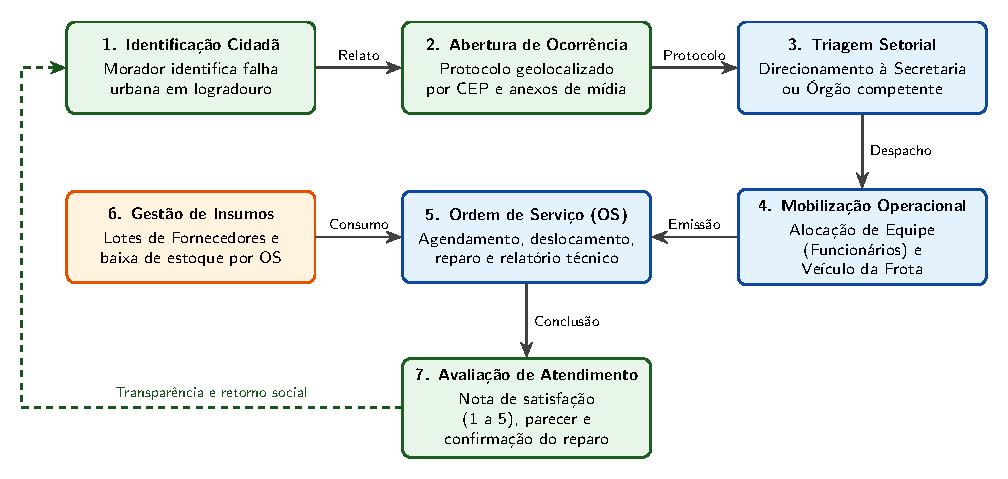
\includegraphics[width=0.95\textwidth]{figuras/fluxo-zeladoria.pdf}
\legend{Fonte: Elaborado pelos autores (2026).}
\end{figure}

\section{Causas Estruturais e Impactos Socioeconômicos, Ambientais e de Saúde}
\label{sec:causas-impactos}

As deficiências observadas decorrem de causas tecnológicas e organizacionais acumuladas na gestão pública local. Destaca-se a prevalência de sistemas departamentais isolados (\emph{silos de dados}), nos quais o registro de atendimento ao cidadão não se comunica com o controle de frotas, recursos humanos e almoxarifado \cite{ibge2024munic}, somada à ausência de padronização territorial por CEP e de indicadores de desempenho que orientem a manutenção preventiva.

Os impactos dessa desarticulação atingem múltiplas dimensões da vida coletiva. Na segurança viária e mobilidade, buracos e semáforos apagados elevam o índice de sinistros de trânsito e causam danos materiais à frota circulante. Na segurança pública e inclusão social, ruas com iluminação inoperante agravam a vulnerabilidade à violência noturna, restringindo a circulação de mulheres, idosos e trabalhadores \cite{ipea2019ods11, ibge2025entorno}. No campo ambiental e de saúde pública, o acúmulo de entulho favorece vetores de arboviroses (como a dengue) e, ao obstruir bocas de lobo, desencadeia alagamentos e exposição a doenças de veiculação hídrica \cite{snis2023drenagem, snis2023residuos}. Economicamente, a demora em executar pequenos reparos multiplica o custo final de reconstrução do pavimento e das galerias.

\section{Atores Envolvidos no Ecossistema de Manutenção Urbana}
\label{sec:atores-envolvidos}

O ecossistema de manutenção urbana congrega cinco grupos de atores que produzem, gerenciam ou utilizam os dados do domínio \cite{heuser2009projeto}: (i) o \textbf{cidadão (morador)}, que identifica a anomalia, abre a ocorrência geolocalizada por CEP com fotos ou vídeos e avalia a resolução após o reparo; (ii) as \textbf{secretarias e órgãos municipais}, que administram o orçamento mensal, coordenam equipes e mantêm a frota; (iii) as \textbf{equipes de manutenção e seus funcionários} (engenheiros, eletricistas, calceteiros), que executam as Ordens de Serviço em campo; (iv) os \textbf{gestores de almoxarifado e frota}, que controlam o estoque de insumos e a disponibilidade dos veículos; e (v) os \textbf{fornecedores terceirizados}, empresas contratadas que entregam lotes de materiais à prefeitura. A Tabela~\ref{tab:atores-sistema} resume o papel e as lacunas enfrentadas por cada ator.

\begin{table}[htb]
\ABNTEXfontereduzida
\caption{Atores envolvidos no ciclo de manutenção urbana, papéis informacionais e dificuldades enfrentadas no modelo tradicional}
\label{tab:atores-sistema}
\centering
\begin{tabular}{L{2.7cm} L{4.2cm} L{4.0cm} L{3.3cm}}
\toprule
\textbf{Ator} & \textbf{Papel no Processo} & \textbf{Dados Produzidos ou Utilizados} & \textbf{Principal Lacuna no Fluxo Tradicional} \\
\midrule
Cidadão (Morador) & Identifica falhas urbanas no território, abre ocorrências e audita o resultado do reparo & Cadastro pessoal, CEP de moradia, relato da ocorrência, mídias e avaliação de atendimento & Falta de retorno sobre o protocolo e impossibilidade de avaliar a solução \\
Secretarias e Órgãos Municipais & Coordenam equipes, gerenciam frota e controlam a execução do orçamento mensal da pasta & Dados da secretaria, orçamento mensal, indicadores de gravidade, custos de OS e avaliações & Visão fragmentada das demandas por bairro e dos gastos reais por reparo \\
Equipes e Funcionários de Campo & Deslocam-se aos locais das ocorrências e executam os reparos técnicos agendados & Turno, disponibilidade, matrícula, cargo, Ordem de Serviço, veículo alocado e relatório técnico & Endereços imprecisos em campo e falta de triagem prévia por imagem \\
Gestão de Almoxarifado e Frota & Controla o estoque de materiais e o estado de conservação dos veículos operacionais & Catálogo de insumos, saldo em estoque, custo médio, baixas por OS e status de veículos & Baixas manuais sem vínculo com a OS e risco de ruptura de estoque \\
Fornecedores Terceirizados & Suprem a prefeitura com insumos de manutenção por meio de lotes contratados & CNPJ, razão social, número de lote de compra, data de entrega, quantidade e preço unitário & Dificuldade de rastrear lotes entregues e variação histórica de preços \\
\bottomrule
\end{tabular}
\legend{Fonte: Elaborado pelos autores (2026).}
\end{table}

\section{Soluções Existentes, Marco Legal e Lacunas Persistentes}
\label{sec:solucoes-lacunas}

No Brasil, o dever estatal de manutenção urbana participativa ampara-se na Lei n\textsuperscript{o}~10.257/2001 (\emph{Estatuto da Cidade}) \cite{brasil2001estatutocidade}, que consagra a gestão democrática da cidade e o direito à infraestrutura urbana, e na Lei n\textsuperscript{o}~13.460/2017 (\emph{Código de Defesa dos Usuários dos Serviços Públicos}) \cite{brasil2017lei13460}, que exige o registro informatizado de manifestações e a avaliação continuada dos serviços públicos por indicadores de satisfação. Embora diversas prefeituras tenham adotado aplicativos do tipo ``156 digital'' \cite{ibge2024munic}, a maioria restringe-se à recepção de chamados (\emph{front-office}), sem modelar a operação de engenharia e suprimentos (\emph{back-office}): inexistem vínculos relacionais entre a ocorrência aberta pelo cidadão, a Ordem de Serviço executada, a equipe e o veículo mobilizados, os lotes de compra de fornecedores e a baixa individualizada de materiais consumidos no reparo.

\section{O Papel Estruturante de um Sistema de Banco de Dados Relacional}
\label{sec:papel-banco-dados}

A superação dessas lacunas requer um banco de dados relacional que assegure integridade referencial, controle de redundância e cruzamento estruturado de dados \cite{elmasri2019sistemas}. No domínio analisado, o banco de dados integra três eixos fundamentais: (i) a \textbf{padronização geográfica e cidadã}, vinculando moradores e ocorrências a uma base única de regiões de CEP e preservando os anexos de mídia comprobatória; (ii) a \textbf{gestão operacional interna}, relacionando secretarias, equipes de manutenção, funcionários e veículos da frota às Ordens de Serviço geradas para cada ocorrência; e (iii) a \textbf{rastreabilidade de insumos e auditoria social}, controlando os lotes de compra entregues por fornecedores, o consumo de materiais em cada Ordem de Serviço e a avaliação final de satisfação registrada pelo cidadão solicitante.

\chapter{Enquadramento nos Objetivos de Desenvolvimento Sustentável (ODS)}
\label{cap:ods}

A Agenda 2030 para o Desenvolvimento Sustentável, adotada em 2015 pelos 193 Estados-membros da Organização das Nações Unidas (ONU), estabelece 17 Objetivos de Desenvolvimento Sustentável (ODS) e 169 metas voltadas a promover o desenvolvimento econômico, social e ambiental integrado \cite{onu2015agenda2030}. Este capítulo fundamenta o enquadramento do problema de monitoramento e manutenção colaborativa de infraestrutura urbana nos compromissos da Agenda 2030, detalhando o ODS principal, suas metas e indicadores oficiais, bem como os dois ODS secundários aos quais o sistema se articula.

\section{ODS Principal: ODS 11 --- Cidades e Comunidades Sustentáveis}
\label{sec:ods-principal}

O problema abordado neste trabalho enquadra-se de maneira central e direta no \textbf{Objetivo de Desenvolvimento Sustentável 11 (ODS 11 --- Cidades e Comunidades Sustentáveis)}, cujo propósito oficial definido pelas Nações Unidas consiste em \emph{``tornar as cidades e os assentamentos humanos inclusivos, seguros, resilientes e sustentáveis''} \cite{onubrasil2015ods11}. Como 87,4\% da população brasileira habita áreas urbanas \cite{ibge2024censo2022malha}, a sustentabilidade das cidades depende diretamente da capacidade municipal de conservar as vias públicas, garantir o funcionamento contínuo dos serviços básicos de zeladoria e instituir canais permanentes de participação cidadã no cuidado com o território \cite{ipea2019ods11}. A aderência estrutural do sistema proposto ao ODS 11 materializa-se prioritariamente nas \textbf{Metas 11.3 e 11.7}, além de dialogar diretamente com a \textbf{Meta 11.6} \cite{onubrasil2015ods11, ipea2019ods11}.

\subsection{Aderência à Meta 11.3 e ao Indicador 11.3.2 (Gestão Urbana Participativa e Integrada)}
\label{subsec:meta-11-3}

De acordo com a redação oficial da Agenda 2030 no Brasil \cite{onubrasil2015ods11}, a \textbf{Meta 11.3} estabelece o seguinte compromisso:

\begin{citacao}
\textbf{Meta 11.3} --- Até 2030, aumentar a urbanização inclusiva e sustentável, e as capacidades para o planejamento e gestão de assentamentos humanos participativos, integrados e sustentáveis, em todos os países \cite{onubrasil2015ods11}.
\end{citacao}

No quadro de monitoramento acompanhado pelo \citeonline{ipea2019ods11}, essa meta é mensurada pelo \textbf{Indicador 11.3.2}, definido como a \emph{``proporção de cidades com uma estrutura de participação direta da sociedade civil no planejamento e gestão urbana que opera de forma regular e democrática''}. O sistema proposto atende diretamente à Meta 11.3 e ao Indicador 11.3.2 ao converter cada morador cadastrado em agente ativo da gestão urbana, permitindo a abertura de ocorrências geolocalizadas por CEP com anexos de mídia e conferindo-lhe o poder de avaliar a qualidade do reparo executado. Simultaneamente, amplia a capacidade de gestão integrada das prefeituras ao conectar as demandas cidadãs ao orçamento das secretarias, às equipes de campo, à frota e ao almoxarifado.

\subsection{Aderência à Meta 11.7 e aos Indicadores 11.7.1 e 11.7.2 (Espaços Públicos Seguros e Acessíveis)}
\label{subsec:meta-11-7}

De modo convergente, a \textbf{Meta 11.7} do ODS 11 volta-se à conservação qualificada e à segurança dos logradouros de uso comum, conforme texto oficial da \citeonline{onubrasil2015ods11}:

\begin{citacao}
\textbf{Meta 11.7} --- Até 2030, proporcionar o acesso universal a espaços públicos seguros, inclusivos, acessíveis e verdes, particularmente para as mulheres e crianças, pessoas idosas e pessoas com deficiência \cite{onubrasil2015ods11}.
\end{citacao}

A Meta 11.7 associa-se ao \textbf{Indicador 11.7.1} (\emph{proporção média da área construída das cidades que é espaço público aberto para uso de todos, por sexo, idade e pessoas com deficiência}) e ao \textbf{Indicador 11.7.2} (relativo à segurança nos espaços públicos) \cite{ipea2019ods11}. Conforme revelam os dados do Censo Demográfico 2022 \cite{ibge2025entorno}, a existência física de uma via não assegura seu uso seguro e inclusivo quando o pavimento está esburacado, a iluminação pública está queimada ou os semáforos encontram-se inoperantes. Ao priorizar por gravidade o reparo de iluminação LED, pavimentação e sinalização viária, o banco de dados promove diretamente a segurança noturna e a acessibilidade nos espaços públicos.

\subsection{Articulação Complementar no ODS 11: Meta 11.6 (Resíduos e Drenagem Urbana)}
\label{subsec:meta-11-6}

Dentro do próprio ODS 11, destaca-se ainda a articulação com a \textbf{Meta 11.6} (\emph{``Até 2030, reduzir o impacto ambiental negativo per capita das cidades, inclusive prestando especial atenção à qualidade do ar, gestão de resíduos municipais e outros''} \cite{onubrasil2015ods11}), monitorada pelo \textbf{Indicador 11.6.1}. Como o sistema contempla o registro geolocalizado de pontos de descarte irregular de entulho e de obstruções na rede de drenagem pluvial \cite{snis2023drenagem, snis2023residuos}, sua operação apoia a erradicação de focos de poluição e alagamentos urbanos.

\section{Enquadramento em ODS Secundários (ODS 9 e ODS 16)}
\label{sec:ods-secundarios}

Além de sua vinculação primária ao ODS 11, o projeto estabelece sinergias diretas com dois objetivos secundários da Agenda 2030:

\begin{itemize}
    \item \textbf{ODS 9 --- Indústria, Inovação e Infraestrutura (Meta 9.1)}: cujo lema consiste em \emph{``construir infraestruturas resilientes, promover a industrialização inclusiva e sustentável e fomentar a inovação''} \cite{onubrasil2015ods9}. O sistema atua diretamente na \textbf{Meta 9.1} (\emph{``Desenvolver infraestrutura de qualidade, confiável, sustentável e resiliente, incluindo infraestrutura regional e transfronteiriça, para apoiar o desenvolvimento econômico e o bem-estar humano, com foco no acesso equitativo e a preços acessíveis para todos''} \cite{onubrasil2015ods9}), garantindo a manutenção contínua e o controle técnico de insumos, equipes e frotas que preservam a confiabilidade da infraestrutura municipal;
    \item \textbf{ODS 16 --- Paz, Justiça e Instituições Eficazes (Metas 16.6 e 16.7)}: voltado a construir instituições eficazes, responsáveis e inclusivas \cite{onubrasil2015ods16}. Ao rastrear o orçamento mensal das secretarias, os custos de mão de obra das Ordens de Serviço, os lotes de compra de fornecedores e a avaliação cidadã do atendimento, o banco de dados materializa a \textbf{Meta 16.6} (\emph{``Desenvolver instituições eficazes, responsáveis e transparentes em todos os níveis''}) e a \textbf{Meta 16.7} (\emph{``Garantir a tomada de decisão responsiva, inclusiva, participativa e representativa em todos os níveis''}) \cite{onubrasil2015ods16}, em consonância com a Lei n\textsuperscript{o}~13.460/2017 \cite{brasil2017lei13460}.
\end{itemize}

A Tabela~\ref{tab:enquadramento-ods} consolida a correspondência entre os ODS, suas metas e indicadores oficiais e as funcionalidades do sistema proposto.

\begin{table}[htb]
\ABNTEXfontereduzida
\caption{Matriz de enquadramento do problema e do sistema proposto nos Objetivos de Desenvolvimento Sustentável da Agenda 2030}
\label{tab:enquadramento-ods}
\centering
\begin{tabular}{L{2.7cm} L{1.8cm} L{4.2cm} L{5.5cm}}
\toprule
\textbf{ODS / Nível} & \textbf{Meta / Indicador} & \textbf{Foco Oficial na Agenda 2030} & \textbf{Materialização no Escopo do Sistema} \\
\midrule
\textbf{ODS 11} \newline Cidades e Comunidades Sustentáveis \newline \emph{(Principal)} & Meta 11.3 \newline Ind. 11.3.2 & Urbanização inclusiva e capacidade de planejamento e gestão participativa e integrada & Abertura de ocorrências pelo cidadão por CEP com envio de mídias, integração entre secretarias e avaliação social do serviço \\
\addlinespace
\textbf{ODS 11} \newline Cidades e Comunidades Sustentáveis \newline \emph{(Principal)} & Meta 11.7 \newline Ind. 11.7.1 \newline Ind. 11.7.2 & Acesso universal a espaços públicos seguros, inclusivos e acessíveis para grupos vulneráveis & Priorização por gravidade de reparos em iluminação pública, pavimentação, calçadas e semáforos para segurança viária e pedonal \\
\addlinespace
\textbf{ODS 11} \newline Cidades e Comunidades Sustentáveis \newline \emph{(Principal)} & Meta 11.6 \newline Ind. 11.6.1 & Redução do impacto ambiental negativo das cidades e gestão adequada de resíduos municipais & Mapeamento e remoção de pontos de descarte irregular de entulho e desobstrução de redes de drenagem pluvial \\
\midrule
\textbf{ODS 9} \newline Indústria, Inovação e Infraestrutura \newline \emph{(Secundário)} & Meta 9.1 & Desenvolvimento e conservação de infraestrutura confiável, sustentável, resiliente e de qualidade & Controle técnico de Ordens de Serviço, equipes especializadas, veículos da frota e insumos de manutenção urbana \\
\addlinespace
\textbf{ODS 16} \newline Paz, Justiça e Instituições Eficazes \newline \emph{(Secundário)} & Metas 16.6 e 16.7 & Instituições públicas eficazes, transparentes e tomada de decisão responsiva e participativa & Rastreabilidade de orçamento mensal, custos de mão de obra, lotes de fornecedores, baixa de estoque e auditoria cidadã \\
\bottomrule
\end{tabular}
\legend{Fonte: Elaborado pelos autores com base em \citeonline{onubrasil2015ods11}, \citeonline{onubrasil2015ods9}, \citeonline{onubrasil2015ods16} e \citeonline{ipea2019ods11}.}
\end{table}

\chapter{Escopo do Sistema de Banco de Dados}
\label{cap:escopo}

Com base na caracterização do problema de zeladoria urbana e em seu alinhamento às metas dos Objetivos de Desenvolvimento Sustentável, este capítulo delimita o escopo de alto nível do sistema de banco de dados relacional proposto. Seguindo a metodologia de projeto de banco de dados preconizada por \citeonline{elmasri2019sistemas} e \citeonline{heuser2009projeto}, apresenta-se aqui a especificação conceitual do minimundo: os subdomínios funcionais, as principais entidades de negócio, as regras de negócio estruturantes e as consultas gerenciais e operacionais que o sistema deve responder. O detalhamento completo dos atributos, chaves identificadoras, cardinalidades no padrão brModelo e o mapeamento para o esquema relacional compõem o escopo específico da Etapa 2 deste projeto.

\section{Visão Geral do Minimundo e Subdomínios Funcionais}
\label{sec:subdominios}

O banco de dados gerencia, de maneira integrada e auditável, todo o ciclo de vida do monitoramento e da manutenção colaborativa da infraestrutura urbana municipal. Para organizar a complexidade do domínio sem perda de coesão, o escopo do sistema estrutura-se em três subdomínios funcionais interdependentes: (i) \textbf{Demandas do Cidadão, Base Geográfica e Avaliação Social}, que abrange a padronização territorial por Código de Endereçamento Postal (CEP), o cadastro dos moradores, a abertura de ocorrências geolocalizadas com arquivos de mídia comprobatória e a avaliação final de satisfação; (ii) \textbf{Estrutura Operacional, Recursos Humanos e Frota Municipal}, que contempla a organização das secretarias e órgãos da prefeitura, a coordenação das equipes de manutenção por categoria e turno, os funcionários operacionais e a frota de veículos; e (iii) \textbf{Execução de Ordens de Serviço, Almoxarifado e Cadeia de Suprimentos}, que compreende o ciclo das Ordens de Serviço (OS), o catálogo e o saldo de materiais de almoxarifado, o consumo de insumos por reparo e o fornecimento por lotes de compra junto a fornecedores.

\section{Principais Entidades de Negócio}
\label{sec:entidades-negocio}

A representação conceitual do sistema fundamenta-se em \textbf{doze entidades de negócio} principais. No primeiro subdomínio, a entidade \textbf{Região de CEP} (\texttt{regiao\_cep}) estabelece a base geográfica padronizada do município (cidade, bairro, logradouro e referência), servindo de âncora espacial tanto para a residência do \textbf{Cidadão} (\texttt{cidadao}) quanto para a localização da \textbf{Ocorrência} (\texttt{ocorrencia}), chamado formal registrado com protocolo único, categoria do defeito, nível de gravidade e status. A entidade \textbf{Anexo de Mídia} (\texttt{anexo\_midia}) armazena os metadados de fotos ou vídeos comprobatórios enviados no relato, enquanto a \textbf{Avaliação de Atendimento} (\texttt{avaliacao\_atendimento}) registra a nota de satisfação (1 a 5), o comentário e a confirmação de resolução após o reparo.

No segundo subdomínio, a entidade \textbf{Secretaria ou Órgão} (\texttt{secretaria\_orgao}) representa cada pasta municipal (Obras, Iluminação, Limpeza), incluindo seu secretário responsável e orçamento mensal. Cada secretaria coordena instâncias de \textbf{Equipe de Manutenção} (\texttt{equipe\_manutencao}), integradas por servidores modelados na entidade \textbf{Funcionário} (\texttt{funcionario}), além de manter os caminhões e utilitários cadastrados em \textbf{Veículo da Frota} (\texttt{veiculo\_frota}). No terceiro subdomínio, a \textbf{Ordem de Serviço} (\texttt{ordem\_servico}) conecta a ocorrência à equipe e ao veículo destacados, registrando cronologia, relatório técnico e custo de mão de obra; \textbf{Material ou Insumo} (\texttt{material\_insumo}) controla o estoque e o custo médio do almoxarifado; e \textbf{Fornecedor} (\texttt{fornecedor}) identifica as empresas que abastecem a prefeitura. A Tabela~\ref{tab:entidades-escopo} sintetiza as doze entidades.

\begin{table}[htb]
\ABNTEXfontereduzida
\caption{Síntese das doze entidades de negócio que compõem o escopo do banco de dados por subdomínio funcional}
\label{tab:entidades-escopo}
\centering
\begin{tabular}{L{3.2cm} L{4.2cm} L{7.0cm}}
\toprule
\textbf{Subdomínio Funcional} & \textbf{Entidade de Negócio} & \textbf{Papel Conceitual no Sistema de Banco de Dados} \\
\midrule
1. Demandas do Cidadão e Base Geográfica & Região de CEP (\texttt{regiao\_cep}) & Padroniza a base territorial (CEP, cidade, bairro, logradouro e referência) para moradias e ocorrências \\
1. Demandas do Cidadão e Base Geográfica & Cidadão (\texttt{cidadao}) & Representa o morador cadastrado que reporta problemas urbanos e avalia a execução dos serviços \\
1. Demandas do Cidadão e Base Geográfica & Ocorrência (\texttt{ocorrencia}) & Registra o chamado de falha na infraestrutura urbana com protocolo, categoria, gravidade e localização \\
1. Demandas do Cidadão e Base Geográfica & Anexo de Mídia (\texttt{anexo\_midia}) & Armazena metadados de fotos e vídeos comprobatórios vinculados existencialmente a uma ocorrência \\
1. Demandas do Cidadão e Base Geográfica & Avaliação de Atendimento (\texttt{avaliacao\_atendimento}) & Registra o parecer final do cidadão (nota de 1 a 5, comentário e confirmação de solução) sobre a OS \\
\midrule
2. Estrutura Operacional e Recursos Municipais & Secretaria ou Órgão (\texttt{secretaria\_orgao}) & Modela os departamentos municipais gestores de orçamento mensal, equipes de campo e frota \\
2. Estrutura Operacional e Recursos Municipais & Equipe de Manutenção (\texttt{equipe\_manutencao}) & Representa os times operacionais especializados por tipo de problema e alocados por turno \\
2. Estrutura Operacional e Recursos Municipais & Funcionário (\texttt{funcionario}) & Cadastra os servidores e técnicos operacionais vinculados às equipes de manutenção \\
2. Estrutura Operacional e Recursos Municipais & Veículo da Frota (\texttt{veiculo\_frota}) & Controla os veículos operacionais das secretarias usados no deslocamento e transporte de materiais \\
\midrule
3. Execução de OS e Cadeia de Suprimentos & Ordem de Serviço (\texttt{ordem\_servico}) & Formaliza a mobilização de equipe e veículo para reparar uma ocorrência, apurando prazos e custos \\
3. Execução de OS e Cadeia de Suprimentos & Material ou Insumo (\texttt{material\_insumo}) & Mantém o catálogo de materiais de almoxarifado, saldo em estoque e custo unitário médio \\
3. Execução de OS e Cadeia de Suprimentos & Fornecedor (\texttt{fornecedor}) & Identifica as empresas contratadas que fornecem lotes de materiais e insumos à administração \\
\bottomrule
\end{tabular}
\legend{Fonte: Elaborado pelos autores em conformidade com a especificação técnica do projeto (2026).}
\end{table}

\section{Regras de Negócio e Restrições de Integridade do Domínio}
\label{sec:regras-negocio}

O banco de dados incorpora regras de negócio rigorosas para assegurar a consistência semântica do domínio: (i) \textbf{localização padronizada por CEP}, pela qual todo cidadão reside em um CEP cadastrado e toda ocorrência referencia obrigatoriamente o CEP do local do problema; (ii) \textbf{autoria e comprovação}, onde cada ocorrência é aberta por um único cidadão e pode possuir múltiplos anexos de mídia com dependência existencial; (iii) \textbf{subordinação operacional}, em que cada secretaria coordena equipes de manutenção (compostas por funcionários) e mantém sua frota de veículos; (iv) \textbf{mobilização em Ordem de Serviço}, permitindo que uma ocorrência gere uma ou mais Ordens de Serviço, cada qual vinculada a uma ocorrência, uma equipe executora e um veículo de deslocamento; (v) \textbf{controle associativo de materiais e compras}, registrando a quantidade utilizada e a data de baixa de cada insumo consumido por Ordem de Serviço, bem como os múltiplos lotes de compra entregues por fornecedores (discriminados por número de lote, data de entrega, quantidade comprada e preço unitário); e (vi) \textbf{avaliação única por atendimento}, assegurando que cada Ordem de Serviço concluída receba no máximo uma avaliação final registrada pelo cidadão autor do chamado.

\section{Consultas e Questões Gerenciais que o Sistema Deve Responder}
\label{sec:consultas-sistema}

A estruturação dessas entidades e regras (que origina, na Etapa 2, quatorze tabelas relacionais a partir das doze entidades fortes e das duas relações associativas de consumo e fornecimento) permite responder a cinco grupos principais de consultas gerenciais e operacionais: (i) \textbf{diagnóstico geográfico de pontos críticos}, identificando bairros e CEPs com maior incidência de falhas por categoria e nível de gravidade; (ii) \textbf{desempenho e tempo de resposta}, apurando o tempo médio entre abertura da ocorrência, emissão da Ordem de Serviço e conclusão do reparo por secretaria e equipe; (iii) \textbf{execução orçamentária e custo real}, somando o custo de mão de obra das Ordens de Serviço ao valor dos materiais consumidos frente ao orçamento mensal de cada secretaria; (iv) \textbf{gestão de estoque e fornecedores}, auditando insumos com estoque crítico, histórico de preços por lote de compra e utilização da frota; e (v) \textbf{auditoria de satisfação cidadã}, calculando a nota média de atendimento por região e a taxa de ocorrências marcadas pelo morador como não resolvidas.

\chapter{Considerações Finais}
\label{cap:consideracoes}

Este relatório apresentou, em conformidade com os requisitos da Etapa 1 da disciplina de Banco de Dados, a análise detalhada do problema de monitoramento e manutenção colaborativa de infraestrutura urbana nos municípios brasileiros, o seu enquadramento fundamentado nos Objetivos de Desenvolvimento Sustentável (ODS) da Agenda 2030 da Organização das Nações Unidas e a delimitação do escopo conceitual do sistema de banco de dados proposto.

A investigação do contexto nacional, respaldada pelas estatísticas oficiais do Censo Demográfico 2022 \cite{ibge2024censo2022malha, ibge2025entorno} e pelos diagnósticos do Sistema Nacional de Informações sobre Saneamento \cite{snis2023drenagem, snis2023residuos}, evidenciou que a conservação das vias e equipamentos coletivos afeta mais de 174 milhões de moradores urbanos. Constatou-se que os entraves enfrentados pelas prefeituras decorrem sobretudo da fragmentação informacional entre os canais de recepção de chamados e a retaguarda operacional das secretarias municipais, gerando protocolos duplicados, imprecisão geográfica, morosidade no despacho de equipes e frotas, descontrole sobre o consumo de insumos de almoxarifado e ausência de retorno formal ao cidadão solicitante.

Sob a perspectiva da sustentabilidade global e das políticas públicas urbanas, demonstrou-se que a estruturação de um banco de dados relacional para gerir esse ciclo completo responde diretamente ao \textbf{ODS 11 (Cidades e Comunidades Sustentáveis)} \cite{onubrasil2015ods11, ipea2019ods11}, com ênfase nas \textbf{Metas 11.3, 11.6 e 11.7}. De modo complementar, o projeto fortalece a resiliência da infraestrutura municipal preconizada pelo \textbf{ODS 9 (Meta 9.1)} \cite{onubrasil2015ods9} e a transparência e eficácia institucional exigidas pelo \textbf{ODS 16 (Metas 16.6 e 16.7)} \cite{onubrasil2015ods16}, alinhando-se às diretrizes do Estatuto da Cidade \cite{brasil2001estatutocidade} e do Código de Defesa dos Usuários dos Serviços Públicos \cite{brasil2017lei13460}.

Por fim, a definição do escopo do banco de dados organizou o minimundo em três subdomínios coesos --- demandas do cidadão e base geográfica, estrutura operacional municipal e execução de ordens de serviço articulada à cadeia de suprimentos ---, totalizando doze entidades de negócio e duas relações associativas de controle de estoque e compras por lote. Como passo seguinte, o trabalho articula-se diretamente à \textbf{Etapa 2}, dedicada à formalização do Modelo Entidade-Relacionamento (MER) conceitual na notação do brModelo (doze entidades, setenta atributos de entidades, quatorze relacionamentos binários e seis atributos de relacionamentos), seguida do mapeamento de \citeonline{elmasri2019sistemas} para as quatorze tabelas do esquema relacional e sua validação em SQL DDL.


% -----------------------------------------------------------------------------
% ELEMENTOS PÓS-TEXTUAIS
% -----------------------------------------------------------------------------
\postextual

\bibliography{referencias}

\end{document}
